\section{项目功能设计}

\subsection{总体功能说明}

\emph{大雾实验工具}是本组成员 2022 春季学期\textit{程序设计进阶与实践}的大作业项目。
本工具搭建于网页平台,支持任何设备自由访问。
传入实验数据后,本工具立刻完成绘制图像、计算不确定度、生成计算公式一系列操作,
并将最终结果整理成一份 \verb|Word| 文档,下载后即可直接使用。
本工具支持一级大物的所有实验,大大提升了学生们撰写实验报告的效率。
由于本工具只是将传入的实验数据进行自动分析,故不会造成抄袭、造假等学术不端问题。

\subsection{具体功能点说明}

使用本工具时,用户只需输入他们做实验时测量到的原始数据,
而无需任何额外的计算处理,用户所要做的只有按照规定的格式上传 \verb|Excel| 文档。
本工具支持 \verb|xlsx|, \verb|csv| 等各种格式的数据表格。
具体而言,每个实验都会有一张示例数据表供用户参考,如图 \ref{fig:interface} 的界面所示。
用户也可以直接下载示例数据,并直接在它的基础上进行修改。
因此,本工具没有任何学习成本,是一款即点即用、免安装的简单轻应用。

\begin{figure}[htbp]
  \centering
  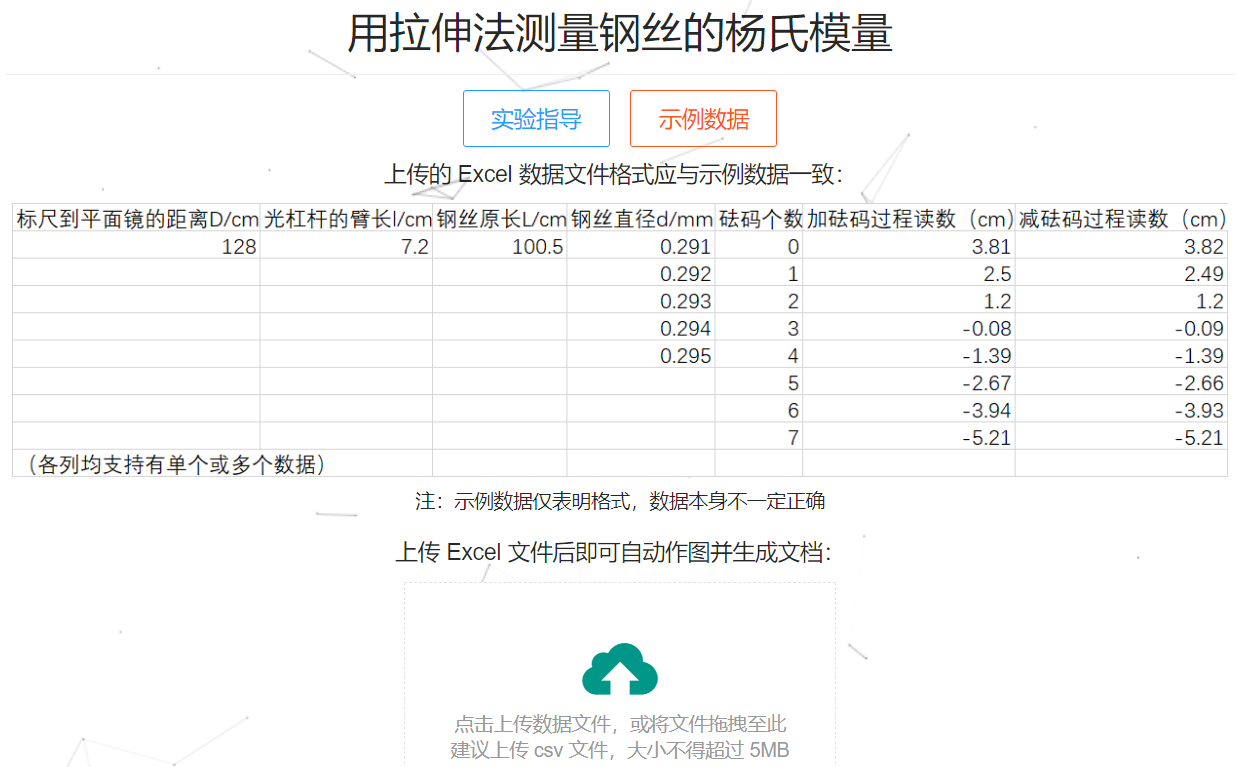
\includegraphics[width=\columnwidth]{figure/interface.png}
  \caption{“拉伸法测钢丝杨氏模量”的工具界面}
  \label{fig:interface}
\end{figure}

\subsubsection*{绘制图像}

本工具根据输入的数据以及实验原理,自动生成美观的实验图像。
本工具支持平滑去噪、数据拟合、双 y 图等多种图像生成需求,如图 \ref{fig:draw} 所示。

\begin{figure}[htbp]
  \centering
  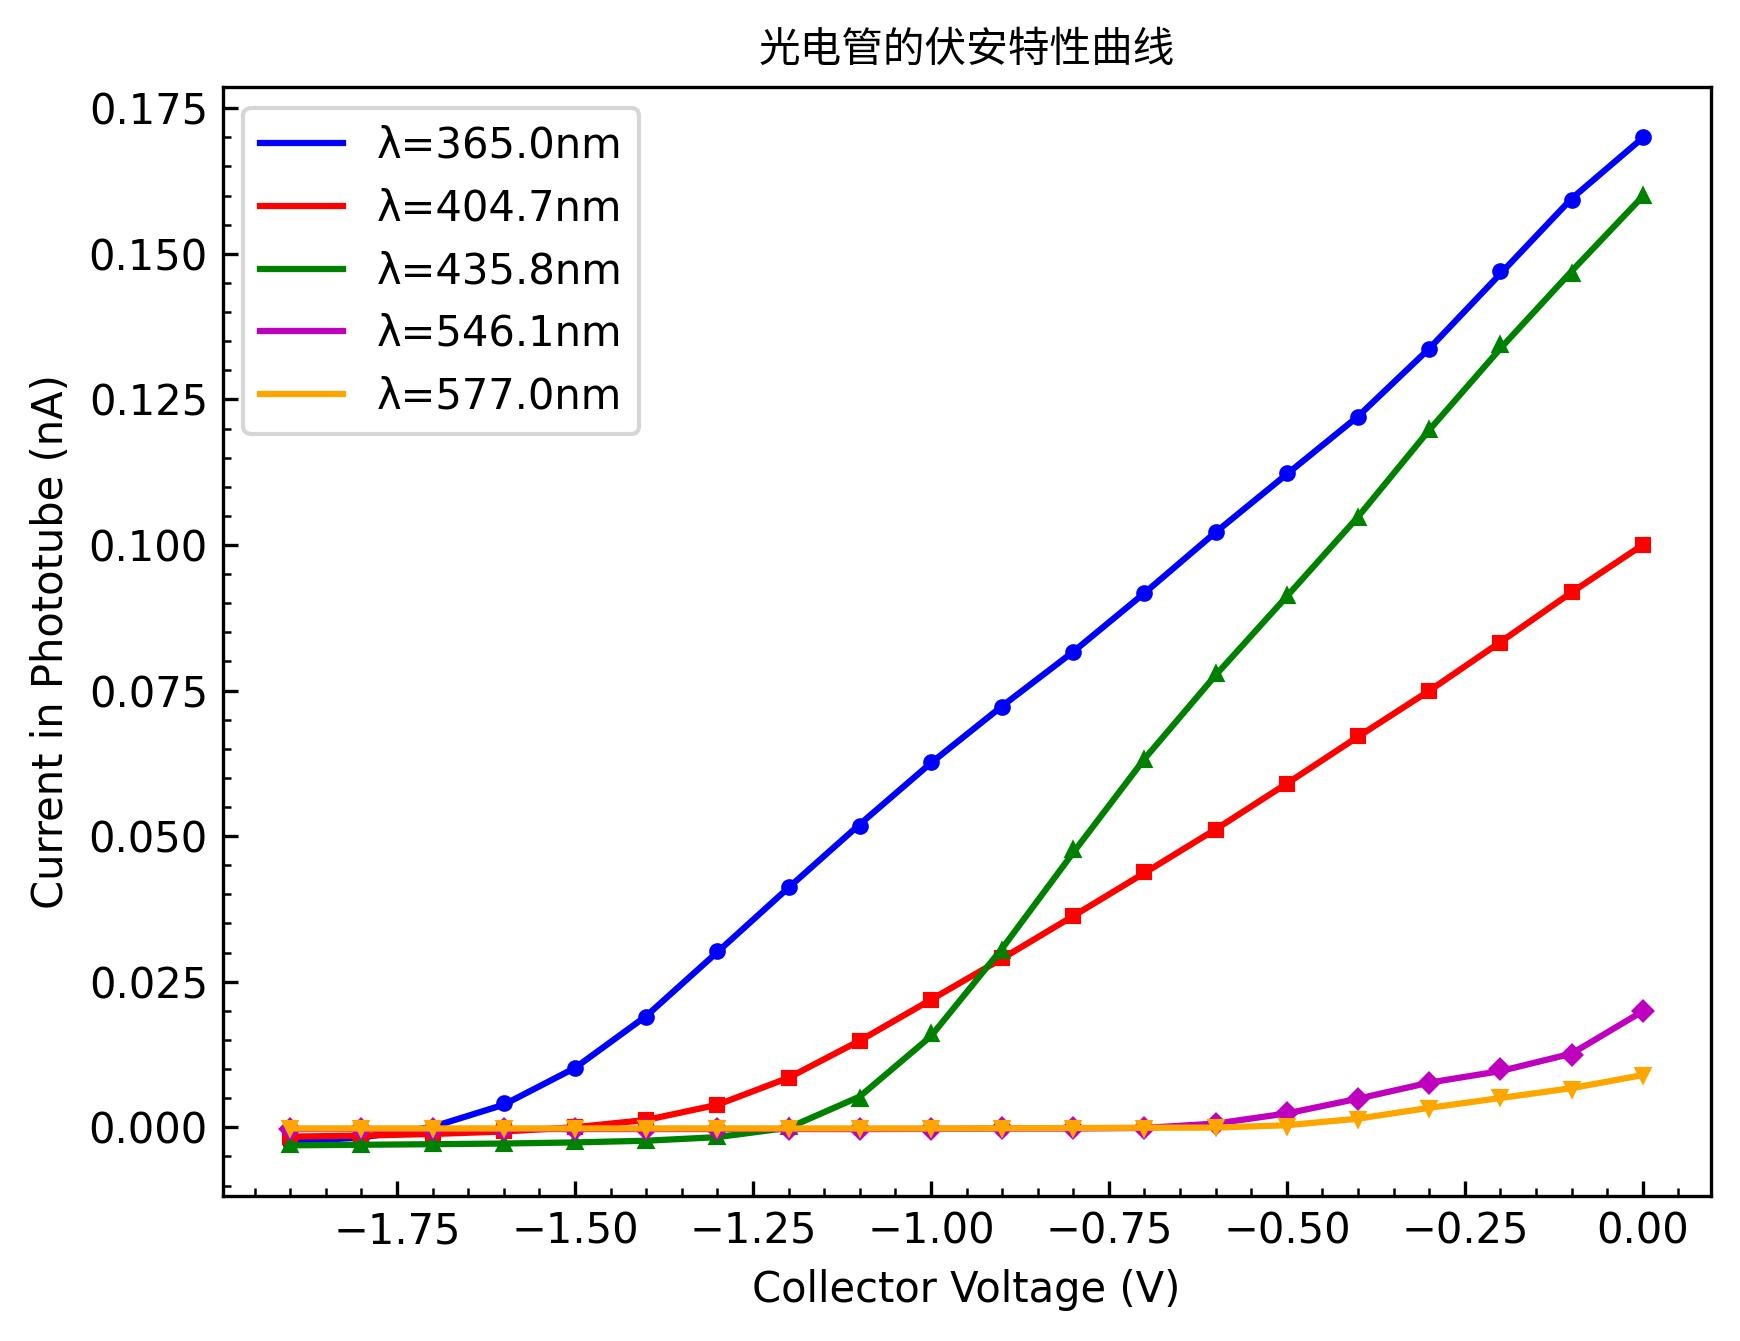
\includegraphics[width=\columnwidth]{figure/draw.jpg}
  \caption{平滑连接的光电效应伏安特性曲线}
  \label{fig:draw}
\end{figure}

\subsubsection*{计算不确定度}

本工具在生成的 \verb|Word| 文档中渲染了各种公式,如图 \ref{fig:calc} 所示。
用户可以直观看到不确定度每一步的计算过程,并在自己的报告中直接使用这些算式与结果。

\begin{figure}[htbp]
  \centering
  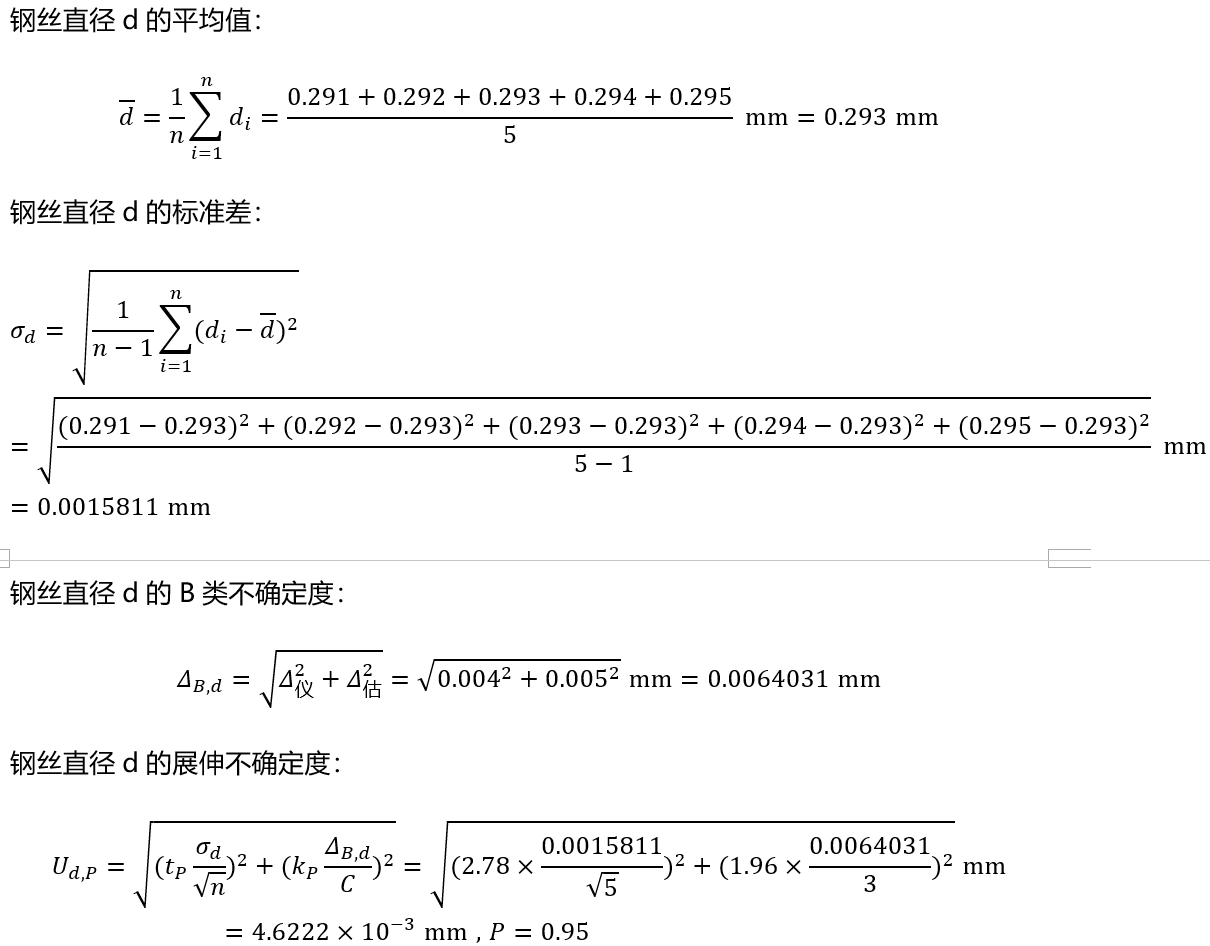
\includegraphics[width=\columnwidth]{figure/calc.png}
  \caption{不确定度计算的详细过程}
  \label{fig:calc}
\end{figure}

\subsubsection*{生成计算公式}

在 \verb|Word| 文档中除了有已经渲染好的公式外,
我们还提供了它们的\LaTeX源码,如图 \ref{fig:latex} 所示。
这极大方便了用\LaTeX, Markdown 等排版实验报告的用户,他们再也不需要手动敲入每一个算式了。

\begin{figure}[htbp]
  \centering
  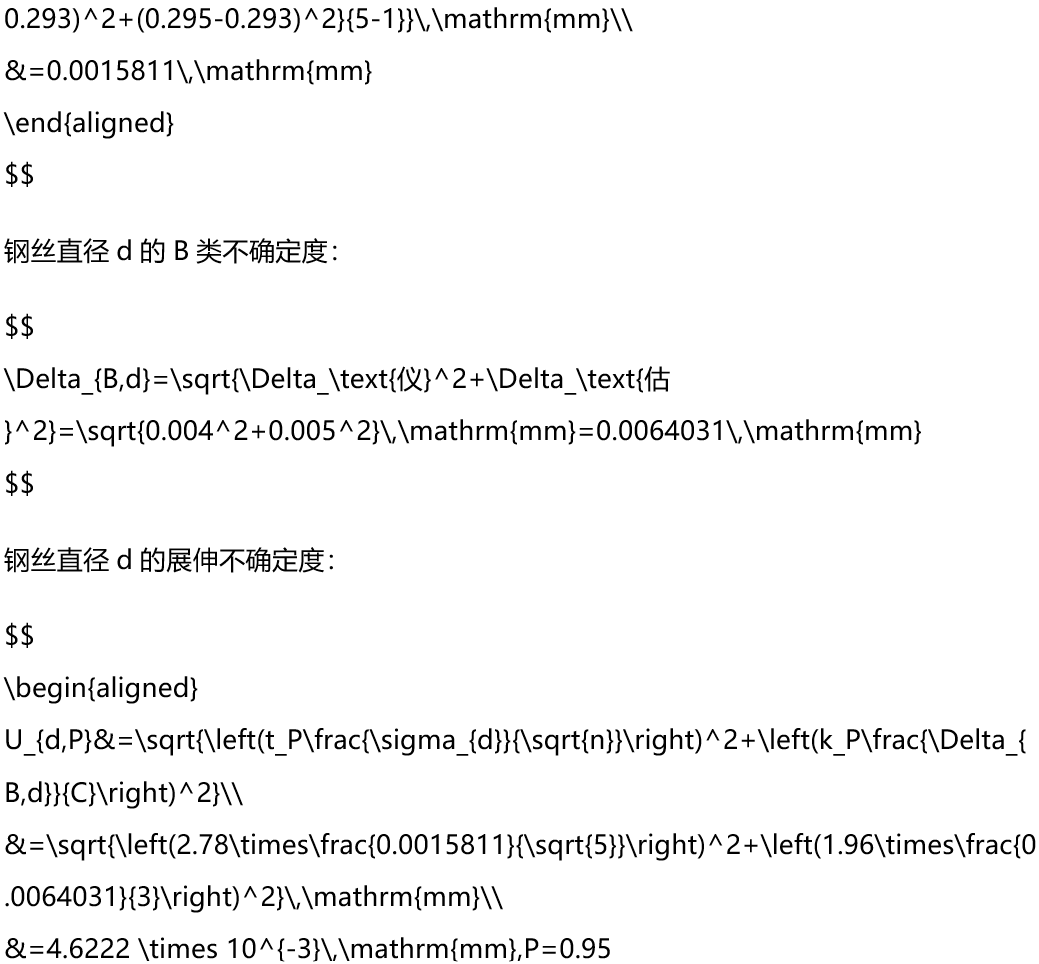
\includegraphics[width=\columnwidth]{figure/latex.png}
  \caption{不确定度算式的\LaTeX源码}
  \label{fig:latex}
\end{figure}

\subsection{功能点设计细节}
